% Section content template for individual Educative lessons
% This file contains the actual content for a specific section
% Generated from Educative API section content

% Section: Evaluation of CDN’s Design
% Section ID: 5971383947624448
% Section Slug: evaluation-of-cdns-design
% Generated: 2025-12-07T17:14:29.201381

\subsection{Requirements compliance}\label{SasVMLw-TVat8uPyZZb-c}
\\
Here, we see how our design fulfills the requirements we discussed in the previous lessons. Our main requirements are high performance, availability, scalability, reliability, and security. Let 's discuss them all one by one.

\subsubsection{Performance}\label{Qp04paCoefykvXxqV-aTN}
\\
CDN achieves high performance by minimizing latency. Some of the key design decisions that minimize latency are as follows:

\begin{itemize}
\item
\protect\phantomsection\label{FZEK9zKH4ZjNwENmbt1hQ}
Proxy servers usually serve content from the RAM.
\item
\protect\phantomsection\label{UoCMR8KRFIpIjdO3AyQwg}
CDN proxy servers are placed near the users to provide faster access to content.
\item
\protect\phantomsection\label{orSB4_ZKAqv4LGUU0qm9w}
A CDN can also be the provider of proxy servers located in the ISP or \textbf{Internet exchange points (IXPs)} to handle high traffic.
\item
\protect\phantomsection\label{W9uuAtePlMqrZGICFHqYr}
The request routing system ensures that users are directed to the nearest proxy servers, as \href{https://www.educative.io/courses/grokking-the-system-design-interview/design-of-a-cdn\#CDN-components}{discussed earlier}.
\item
\protect\phantomsection\label{LKBa3iQKDAJVqlk0S3Hnc}
The proxy servers have long-tail(If we monitor the access frequency of our content over some time, we can see a trend where some content is read by many clients (for example, 20\% of content asked by 80\% of clients), and then there is a long list of the content that very few clients ask for. Such an access distribution is called a long-tailed distribution.) content stored in nonvolatile storage systems like SSD or HDD. Serving from these resources results in a more negligible latency than we'd see from serving content from origin servers.
\end{itemize}

\begin{figure}[htbp]
 \centering
 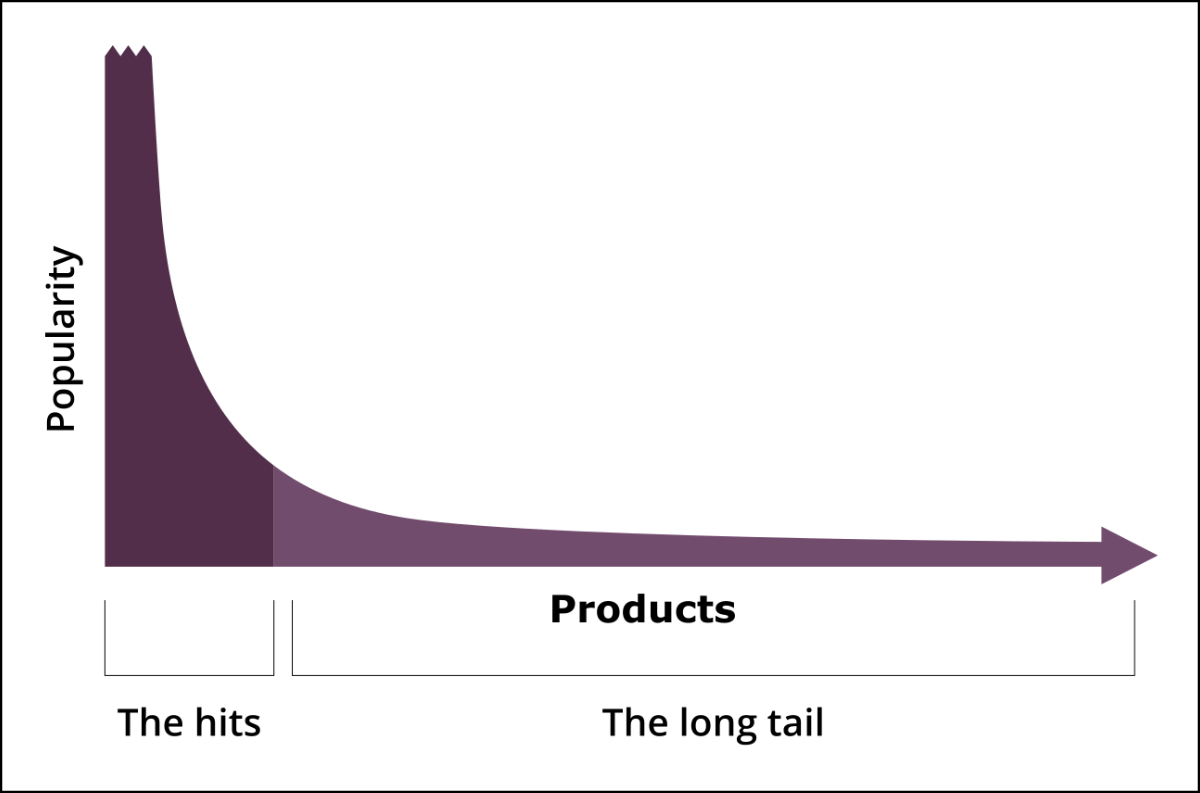
\includegraphics[width=0.5\textwidth]{Images/chapter_11/section_5971383947624448/6622644521009152.png}
 \caption{Many kinds of data exhibit the long-tailed phenomenon}
\end{figure}

\begin{itemize}
\item
\protect\phantomsection\label{oLGti32hxmWqzBVcBYjDS}
As was discussed previously, proxy servers can be implemented in layers where if one layer doesn't have the content, the request can be entertained by the next layer of proxy servers. For example, the edge proxy servers can request the parent proxy servers. Placing proxy servers at specific ISPs could be the best option when most traffic comes from those ISP regions.
\end{itemize}
\\
\paragraph{Availability}\label{kCI7yfsG2X0Ht2Dx2BPsC}
\\
A CDN can deal with massive traffic due to its distributed nature. A CDN ensures availability through its cached content that serves as a backup whenever the origin servers fail. Moreover , if one or more proxy servers in the CDN stop working, other operational proxy servers step in and continue to drive the web traffic. In addition, edge proxy servers can be made available through redundancy by replicating data to as many proxy servers as needed to avoid a single point of failure and to meet the request load. Finally
, we can use a load balancer to distribute the users' requests to nearby active proxy servers.
\\
\paragraph{Scalability}\label{aK3RyKKJW7gf6hpBXPAe7}
\\
The design of CDN facilitates scalability in the following ways:

\begin{itemize}
\item
\protect\phantomsection\label{JvH-Gg8JgWNM3KAdV86do}
It brings content closer to the user and removes the requirement of high bandwidth, thereby ensuring scalability.
\item
\protect\phantomsection\label{rNDLTlEpwD96Kg7dQ_s_w}
Horizontal scalability is possible by adding the number of reading replicas in the form of edge proxy servers.
\item
\protect\phantomsection\label{u2vHUlV19YDKv6nRCcWXt}
The limitations with horizontal scalability and storage capacity of an individual proxy server can be dealt with using the layered architecture of the proxy servers we described above.
\end{itemize}
\\
\paragraph{Reliability and security}\label{Ez43RfkKa4eekncSXytdO}
\\
A CDN ensures no single failure point by carefully implementing maintenance cycles and integrating additional hardware and software when required. Apart from failures, the CDN handles massive traffic loads by equally distributing the load to the edge proxy servers. We can use scrubber servers to prevent DDoS attacks and securely host content. Moreover, we can use the \textbf{heartbeat protocol} to monitor the health of servers and omit faulty servers. Real-time applications also build their own specified CDNs to prevent content leakage problems and securely serve content to their end users.

\subsubsection{Conclusion}\label{yOzLUEumF_Yyqo7LQ2hUb}
\\
Since its inception in the 1990s, the CDN has played a vital role in providing high availability and low-latency content delivery. Nowadays , CDNs are considered a key player in improving the overall performance of giant services.\\
\strut \\

% End of section content